\section{Implementacija upoređivača}
\label{sec:ImplementationComparer}

Implementacija algoritma upoređivača opisana u poglavlju \ref{chp:ASTComparing} se svodi na implementaciju funkcija za poređenje za svaki tip AST čvora. Te funkcije su enkapsulirane u klase koje implementiraju interfejs za upoređivač čvorova. Te klase nisu javne, tako da se poređenje vrši kroz upoređivač koji poredi instance tipa \texttt{ASTNode}, a koji putem refleksije određuje konkretni tip čvorova i, ukoliko su tipovi isti, pronalazi konkretni upoređivač i poziva operaciju interfejsa upoređivača. Upoređivači međusobno pozivaju jedni druge, kako bi se logika poređenja uprostila - pošto se naredbe deklaracije sastoje od specifikatora deklaracije i liste deklaratora, upoređivač naredbi deklaracije može pozivati upoređivač za specifikatore deklaracije i upoređivač za listu deklaratora. Rezultat rada upoređivača za algoritam \emph{swap} se može videti na slici \ref{fig:ComparerSwap}.

\begin{figure}[h!]
\centering
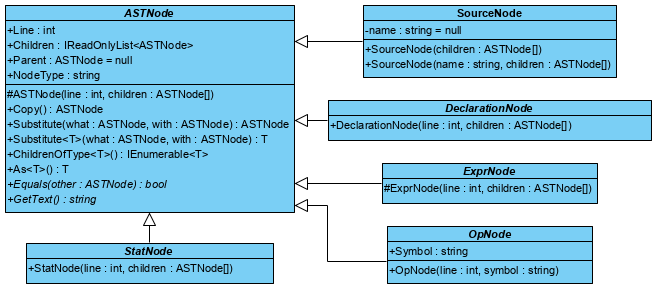
\includegraphics[scale=0.7]{images/uml/ASTNode.png}
\caption{Rezultat rada upoređivača za \texttt{swap} algoritam.}
\label{fig:UMLASTNode1}
\end{figure}
